\begin{flushright}
    \textit{Лекция 14 (от 20.10)}
\end{flushright}
\section{$\S 18.$ Вычисление интегралов от регулярных ветвей.}
\Example
Вычислить при помощи теории вычетов интеграл
\begin{align*}
  & I = \int_0^2 \frac{\sqrt[4]{x^3(2-x)}}{(1+x)^2} dx
\end{align*}
\nonum
$g(z) = \sqrt[4]{z^3(2-z)}$ дает многозначную функцию. Отыщем регулярные ветви;
рассмотрим область, где ветви существуют. Функция $f(z) = z^3(2-z)$ должна быть
в области регулярной и не равной нулю.
\\
Рассмотрим $\CC \setminus [0;2]$. В такой области этот корень имеет регулярную
ветвь.
\\
Отыщем ветвь, что нам нужна. Построим ее так, чтобы $g(1+i0) = 1$; тогда
$\forall x \in [0;2] \ g(x+i0) = \sqrt[4]{x^3(2-x)}$. В этом случае
\begin{align*}
  & g(x-i0) = g(1+i0)\sqrt[4]{\frac{\left| g(x-i0) \right|}{\left| g(1+i0) \right|}}\exp\left( \frac{i}{4}\left( 3\Delta_{\gamma_{1+i0,x}}\argt z + \Delta_{\gamma_{1+i0,x}}\argt (2-z) \right) \right) = \\
  & = \sqrt[4]{\frac{\left| g(x-i0) \right|}{\left| g(1+i0) \right|}}\exp\left( \frac{-i\pi}{2}\right)
\end{align*}
\begin{figure}[h!]
		\centering
		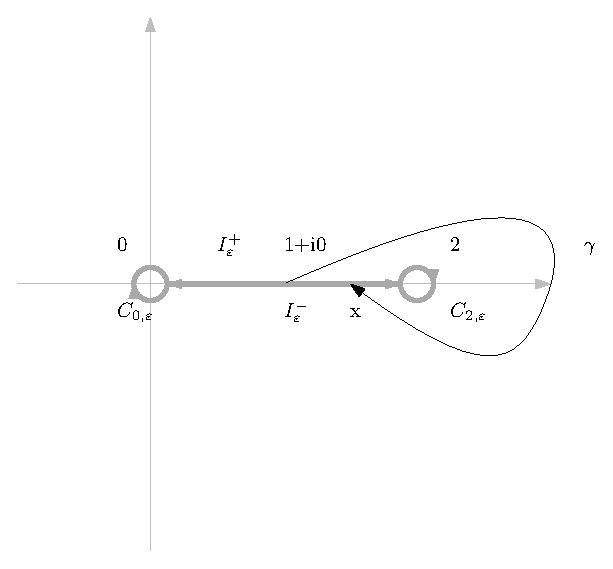
\includegraphics[scale=0.75]{Par18.eps}
		\label{fig:18.1}
\end{figure}
Рассмотрим
\begin{align*}
  & \gamma_\varepsilon = I_\varepsilon^+\cup C_{2, \varepsilon} \cup I_\varepsilon^-\cup C_{0, \varepsilon}
\end{align*}
и
\begin{align*}
  & F(z) = \frac{\sqrt[4]{z^3(2-z)}}{(1+z)^2} = \frac{g(z)}{(1+z)^2}
\end{align*}
и вычислим
\begin{align*}
  & I_\varepsilon = \int_{\gamma_\varepsilon}F(z) dz = 2 i \pi \left( \us{-1}{\res} F(z) + \us{\infty}{\res} F(z) \right)
\end{align*}
Видим, что $-1$~--- полюс $2$ порядка, а $\infty$~--- УОТ.
\begin{align*}
  & \us{-1}{\res} F(z) = \lim_{z \to -1}((z+1)^2F(z))' = \lim_{z \to -1}g'(z) = g'(-1) = \left. \frac{f'(z)}{4g^3(z)}\right|_{z = -1} = \frac{-4(-1)^3+6(-1)^2}{4\left( \sqrt[4]{3}\exp\left( \frac{3i\pi}{4} \right)\right)^3} = \\
  & = \frac{5}{2\sqrt[4]{27}}\exp\left( \frac{-i\pi}{4} \right)
\end{align*}
Рассмотрим $x \in (2; \infty)$; тогда
\begin{align*}
  & g(x) = \sqrt[4]{x^3(2-x)}\exp\left( \frac{-i\pi}{4} \right) = x\sqrt[4]{1-\frac{2}{x}}\exp \left( \frac{-i\pi}{4} \right) = x\exp\left( \frac{-i\pi}{4} \right)\sum_{n=0}^\infty C_{\frac{1}{4}}^n\left( -\frac{2}{x} \right)^n
\end{align*}
Две регулярные функции ($g(x)$ и сумма) совпадают на $(2; \infty)$, а значит, по
теореме единственности
\begin{align*}
  & g(z) = z\exp\left( \frac{-i\pi}{4} \right)\sum_{n=0}^\infty C_{\frac{1}{4}}^n\left( -\frac{2}{z} \right)^n, \ \left| z \right|> 2
\end{align*}
\begin{align*}
  & F(z) = \frac{z}{(z+1)^2}h(z), \ h(z) = \exp\left( \frac{-i\pi}{4} \right)\sum_{n=0}^\infty C_{\frac{1}{4}}^n\left( -\frac{2}{z} \right)^n
\end{align*}
Заметим, что
\begin{align*}
  & \frac{z}{(1+z)^2} = \frac{1}{z(1+\frac{1}{z})^2} = \frac{1}{z} \left( 1-\frac{2}{z} +\frac{3}{z^2} + \dots \right)
\end{align*}
При перемножении двух рядов получим
\begin{align*}
  & \us{\infty}{\res}F(z) = -\exp\left( \frac{-i\pi}{4} \right)
\end{align*}
и интеграл
\begin{align*}
  & I_\varepsilon = 2 i \pi \left( \frac{5}{2\sqrt[4]{27}} - 1 \right)\exp\left( \frac{-i\pi}{4} \right)
\end{align*}
не зависит от $\varepsilon$. Заметим, что
\begin{align*}
  & I_\varepsilon = \int_{I_\varepsilon^+}F(z) + \int_{C_{2, \varepsilon}}F(z) + \int_{I_\varepsilon^-}F(z) + \int_{C_{0, \varepsilon}}F(z)
\end{align*}
Причем
\begin{align*}
  & \int_{I_\varepsilon^+}F(z) = \int_{\varepsilon}^{2-\varepsilon}\frac{\sqrt[4]{x^3(2-x)}}{(x+1)^2}dx
\end{align*}
\begin{align*}
  & \int_{I_\varepsilon^-}F(z) = \int_{2-\varepsilon}^{\varepsilon}\frac{g(x-i0)}{(x+1)^2}dx = -\int_{\varepsilon}^{2-\varepsilon}\frac{\sqrt[4]{x^3(2-x)}\exp\left( \frac{3i\pi}{2} \right)}{(x+1)^2}dx = -\exp\left( \frac{3i\pi}{2}\right) \int_{I_\varepsilon^+}F(z)
\end{align*}
Учтя $z = \varepsilon e^{i \varphi}$,
\begin{align*}
  & \left|  \int_{C_{0, \varepsilon}}F(z) \right| \leq \int_{0}^{2 \pi}\frac{\varepsilon\sqrt[4]{\varepsilon^3(2+\varepsilon)}}{(1-\varepsilon)^2}d\varphi \leq A\varepsilon^{\frac{7}{3}} \us{\varepsilon \to 0}{\to} 0
\end{align*}
Учтя $z = 2 + \varepsilon e^{i \varphi}$,
\begin{align*}
  & \left|  \int_{C_{2, \varepsilon}}F(z) \right| \leq \int_{0}^{2 \pi}\frac{\varepsilon\sqrt[4]{(2+\varepsilon)^3\varepsilon}}{(3-\varepsilon)^2}d\varphi \leq B\varepsilon^{\frac{4}{3}} \us{\varepsilon \to 0}{\to} 0
\end{align*}
Значит,
\begin{align*}
  & 2 i \pi \left( \frac{5}{2\sqrt[4]{27}} - 1 \right)\exp\left( \frac{-i\pi}{4} \right) = I_\varepsilon \us{\varepsilon \to 0}{\to} \int_{I_\varepsilon^+}F(z) + \int_{I_\varepsilon^-}F(z) = \left( 1 -\exp\left( \frac{3i\pi}{2}\right) \right) \int_{I_\varepsilon^+}F(z) \us{\varepsilon \to 0}{\to} \\
  & \us{\varepsilon \to 0}{\to} \left( 1 -\exp\left( \frac{3i\pi}{2}\right) \right) I
\end{align*}
Значит,
\begin{align*}
  & I = \frac{2 i \pi \left( \dst \frac{5}{2\sqrt[4]{27}} - 1 \right)\exp\left( \dst\frac{-i\pi}{4} \right)}{\left( 1 -\exp\left( \dst \frac{3i\pi}{2}\right) \right)}= \pi \sqrt{2}\left( \dst \frac{5}{2\sqrt[4]{27}} - 1 \right)
\end{align*}
\section{$\S 19.$ Целые и мероморфные функции.}
\Def
Функция $f$ называется \textbf{целой}, если она регулярна на $\CC$.
\\
Можем представить такую функцию в виде
\begin{equation}\label{(19.1)}
    \forall z \in \CC \ f(z) = \sum_{n=0}^\infty c_nz^n, \ c_n = \frac{1}{2i\pi}\int_{\gamma_r}\frac{f(\zeta)}{\zeta^{n+1}} d \zeta
\end{equation}
\theorem
Пусть $f:G \mapsto \CC$ целая, $\exists A > 0, \ R > 0, \ m \in \NN_0$ такие,
что $\forall z: \left| z \right| > R \hookrightarrow \left| f(z) \right| \leq
A\left| z \right|^m$. Тогда $f(z)$~--- многочлен степени $\leq m$.
\pr
Воспользуемся оценкой $c_n$.
\begin{align*}
  & \forall r > R \ \left|c_n \right| \leq \frac{1}{2\pi}\int_{\left| \zeta \right| = r} \frac{\left| f(\zeta) \right|}{\left| \zeta \right|^{n+1}}\left| d\zeta \right|\leq \frac{1}{2\pi}\frac{Ar^m}{r^{n+1}}r\cdot 2 \pi = Ar^{m-n}
\end{align*}
Значит, $\forall n > m \ c_n = 0$.
\corollary (теорема Лиувилля)
Если $f$ целая, $\exists R > 0, \ A > 0$: $\left| f(z) \right|< A$ при $\left| z
\right| > R$, то $f \equiv const$.
\theorem (Основная теорема алгебры)
Всякий многочлен $P_n(z) = z^n + C_{n-1}z^{n-1}+\dots+c_0$ имеет в $\CC$ хотя бы
один корень.
\pr
предположим, $\forall z \in \CC \ P_n(z) \neq 0$. Тогда $\varphi(z) = \dst
\frac{1}{P_n(z)}$ целая. Но, как легко видеть,
\begin{align*}
  & \lim_{z \to \infty}P_n(z) = \infty \Rightarrow \lim_{z \to \infty} \varphi(z) = 0 \Rightarrow \exists R > 0: \ \forall z: \ \left| z \right| > R \hookrightarrow \left| \varphi(z) \right| < 1
\end{align*}
Значит, по теореме Лиувилля $\varphi(z) = const$, тогда и $P_n(z) = const$.
Противоречие.
\\
Значит, можем заметить, что для целой функции $f$ единственная особая точка~---
это $\infty$.
\begin{itemize}
    \item $\infty$~--- УОТ, тогда $f = const$.
    \item $\infty$~--- полюс порядка $m$, тогда $f = P_m$.
    \item $\infty$~--- СОТ.
\end{itemize}
\Def
Целая функция, у которой $\infty$ есть СОТ, назвается \textbf{целой
  трансцендентной}.
\theorem (Сохоцкого)
Пусть $f$~--- целая трансцендентная функция, тогда
\begin{align*}
  & \forall A \in \CCC \ \exists z_n \to \infty: \ \lim_{n \to \infty}f(z_n) = A
\end{align*}
\pr
Рассмотрим два случая.
\begin{itemize}
    \item $A = \infty$
    \\
    $f$ неограничена в окрестности $\infty$ (т.~к. иначе она бы имела конечный
    предел), т.~е.
    \begin{align*}
      & \forall n \in \NN \ \exists z_n \in \CC: \left| f(z_n) \right|> n, \ \left| z_n \right| > n
    \end{align*}
    Итак, $\left\{ z_n \right\}$ и есть та самая последовательность.
    \item $A \in \CC$
    \\
    Пусть, от противного,
    \begin{align*}
      & \exists \delta_0 > 0, \ \varepsilon_0 > 0: \ \forall z: \ \left| z \right| \geq \delta_0 \ \left| f(z) - A \right| \geq \varepsilon_0
    \end{align*}
    Пусть $\varphi(z) = \dst \frac{1}{f(z) - A}$, $z \in B_{\delta_0}(\infty)$.
    На этом множестве
    \begin{align*}
      & \left| \varphi(z) \right| \leq \frac{1}{\varepsilon_0}
    \end{align*}
    Значит, эта функция на этом множестве регулярна и ограничена, а значит, для
    нее $\infty$~--- УОТ, т.~е.
    \begin{align*}
      & \exists \lim_{z \to \infty}\varphi(z) = B
    \end{align*}
    Значит, $\infty$~--- полюс либо УОТ для $f(z)$, противоречие.
\end{itemize}
\theorem (общая теорема Сохоцкого)
Пусть $f: \os{\circ}{B}_r(a) \mapsto \CC$ регулярна, $a$~--- СОТ $f$. Тогда
\begin{align*}
  & \forall A \in \CCC \ \exists z_n \to a, \ \lim_{n \to \infty} f(z_n) = A
\end{align*}
\Exse
доказать общую теорему Сохоцкого.
\theorem (Пикара)
Пусть $f$~--- целая трансцедентная функция, тогда $\forall a \in \CC$, за
исключением, быть может, одного, $\exists R > 0$: в $\os{\circ}{B}_R(\infty)$
существует бесконечное число решений уравнения $f(z) = A$, т.~е.
\begin{align*}
  & \exists z_n \to \infty: \ \forall n \in \NN \ f(z_n) = A
\end{align*}
\Example
$e^z = A$ имеет счетное число решений в любой окрестности бесконечности при $A
\neq 0$, но ни одного решения при $A = 0$.
\Exse
Пусть $f$~--- целая функция и
\begin{align*}
  & \exists A > 0, R > 0, \ m \in \NN_0: \ \forall z: \ \left| z \right| > R \ \left| f(z) \right| \geq A \left| z \right|^m
\end{align*}
Доказать, что $f$~--- многочлен степени $\leq m$.
\Def
Функция $f$ называется мероморфной, если $\forall R > 0$ в круге $B_R(0)$ она
регулярна за исключением, быть может, конечного числа полюсов.
\Example
\begin{align*}
  & f(z) = \frac{P_n(z)}{Q_m(z)}
\end{align*}
Конечное число полюсов на всей $\CC$.
\Example
\begin{align*}
  & f(z) = \ctg z
\end{align*}
Счетное число полюсов на $\CC$.
\Example
\begin{align*}
  & f(z) = \frac{z}{e^z-1}
\end{align*}
Счетное число полюсов на $\CC$.